\documentclass[../AnalisideiRequisiti.tex]{subfiles}

\begin{document}
	% Il comando UserCase accetta primo una label nel caso serva un link verso di lui \refer{label} poi 
	% attore primario
	% attore secondario
	% Descrizione
	% Precondi
	% Post
	% Scenario principale
	% Scenari alternativi 

	\chapter{Casi d'uso}
	\section{Classificazione dei casi d'uso}
	I casi d'uso sono identificati da un codice descritto nelle NP alla sezione §2.2.3.4. 
	
 	
	\section{UC0: Avvio Applicazione}
	\begin{figure}[H]
 
		\centering
 
		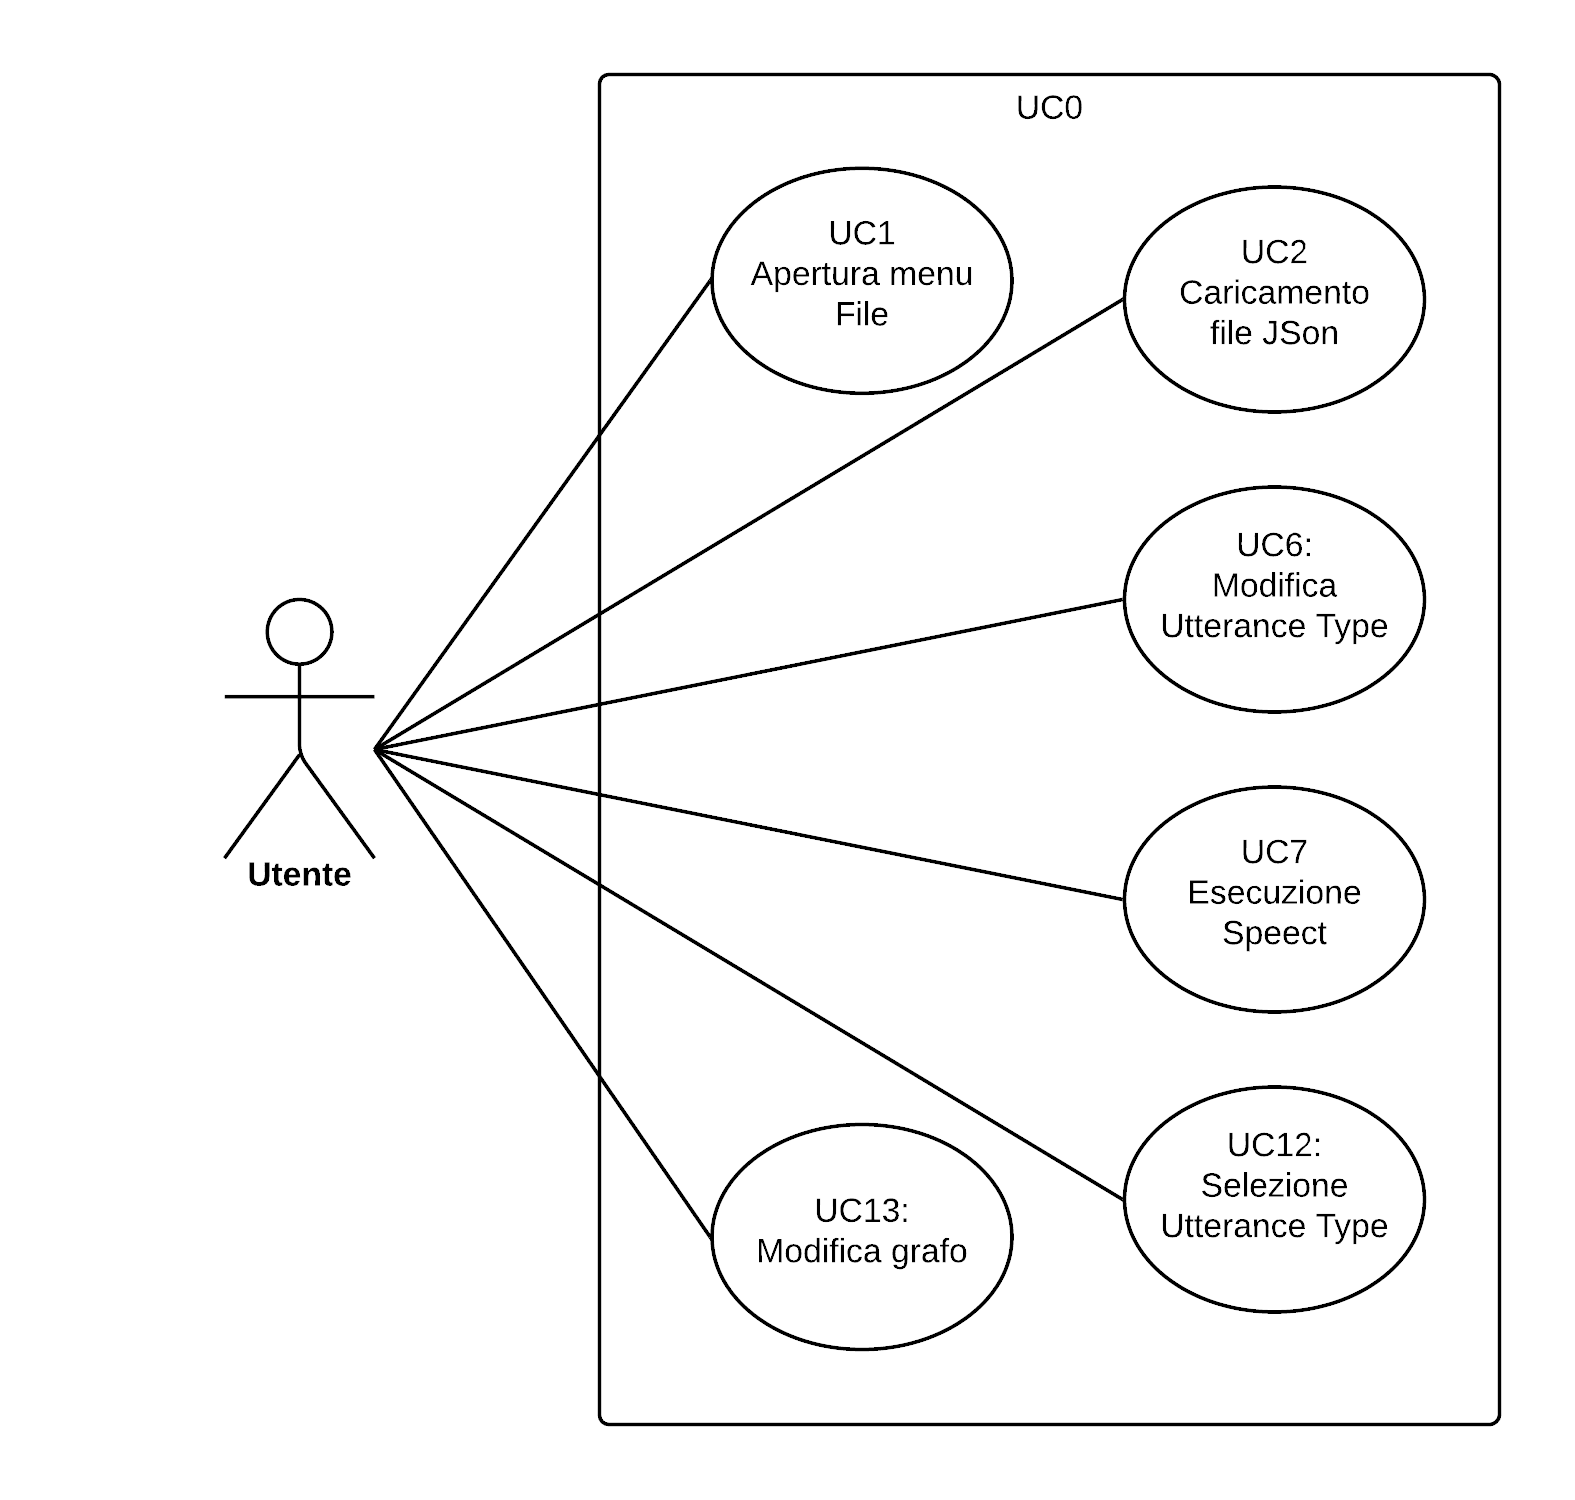
\includegraphics[width=\textwidth]{../img/UC0.png}
 
		\caption{UC0: Avvio Applicazione}
 
	\end{figure}
	\UserCase
	{UC0}
	{Utente}
	{Non previsto}
	{L'attore avvia l'applicazione DeSpeect}
	{Il software Despeect è correttamente installato}
	{L'applicazione è correttamente avviata}
	{Viene visualizzata la pagina iniziale \refer{UC0.1}}
	{Non previsti}
	
	\section{UC0.1: Visualizzazione Pagina Iniziale}
	\UserCase
	{UC0.1}
	{Utente}
	{Non previsto}
	{L'attore visualizza la pagina iniziale}
	{Il software DeSpeect è correttamente avviato \refer{UC0}}
	{L'applicazione visualizza la pagina iniziale}
	{L'applicazione si avvia e l'attore visualizza la pagina iniziale}
	{Non previsti}
	
	\section{UC1: Apertura Menu File}
	\UserCase
	{UC1}
	{Utente}
	{Non previsto}
	{L'attore vuole visualizzare il menu File}
	{L'applicazione è correttamente avviata \refer{UC0}}
	{Vengono visualizzate le voci del menu File}
	{	\begin{enumerate}
			\item{} L'attore preme sul menu File
			\item{} Il menu File si apre e offre le seguenti scelte:
		\begin{itemize}
		\item{} L'attore può caricare un file JSon \refer{UC2}
		\item{} L'attore può salvare le modifiche al file JSon \refer{UC11}
		\item{} L'attore può caricare un grafo \refer{UC8}
		\item{} L'attore può salvare un grafo \refer{UC9}
		\item{} L'attore può salvare l'audio prodotto da Speect \refer{UC4}
		\item{} L'attore può cercare il percorso di un nodo nel grafo \refer{UC10}
		\item{} L'attore può chiudere l'applicazione \refer{UC5}
		\end{itemize}
	\end{enumerate}
	}
	{Non previsti}

	\section{UC2: Caricamento File JSon}
	\begin{figure}[H]
		\centering
		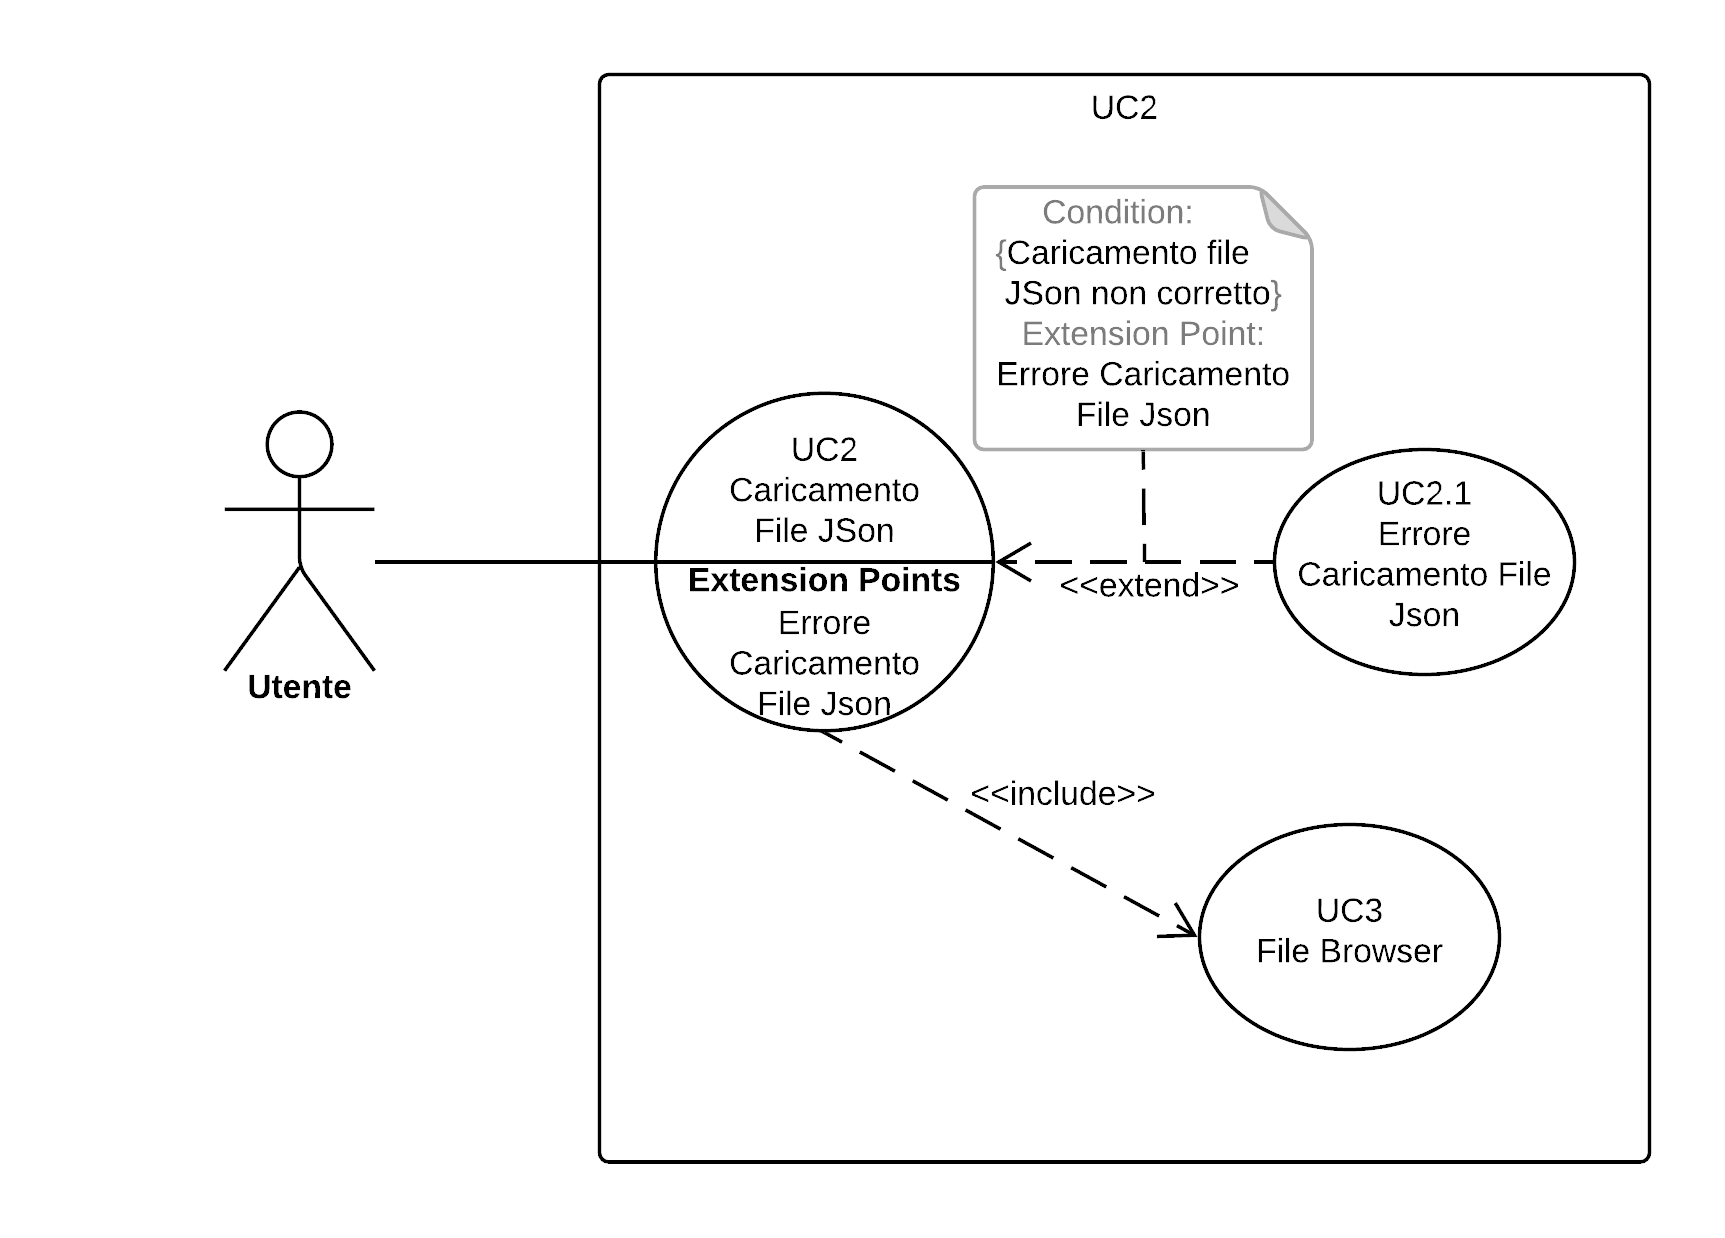
\includegraphics[width=\textwidth]{../img/UC2.png}
		\caption{UC2: Caricamento File JSon}
	\end{figure}
	\UserCase
	{UC2}
	{Utente}
	{Non previsto}
	{L'attore vuole caricare un file JSon}
	{L'attore ha selezionato la voce relativa nel menu \refer{UC1}}
	{Viene inizializzato Speect con il file JSon selezionato e aggiornata la GUI}
	{
		\begin{itemize}
			\item{} Viene aperto il file browser \refer{UC3}
			\item{} L'attore seleziona il file \refer{UC3.2}
			\item{} L'attore preme Carica
			\item{} Il file viene dato a Speect che prova l'inizializzazione
			\item{} Viene visualizzato il percorso del file nell'apposito spazio \ref{fig:GUI}
		\end{itemize}
	}
	{Speect fallisce l'inizializzazione e l'attore visualizza il messaggio dell'errore relativo al file \refer{UC2.1}}
	
	\section{UC2.1: Errore Caricamento File JSon}
	\UserCase
	{UC2.1}
	{Utente}
	{Non previsto}
	{Durante l'inizializzazione Speect fallisce ritornando un errore}
	{L'attore carica un file JSon non corretto}
	{L'errore è visualizzato a schermo e viene ripristinato lo stato precedente ridando controllo all'attore}
	{L'attore ha caricato un file JSon non corretto e viene visualizzato un messaggio di errore}
	{Non previsti}

	\section{UC3: File Browser}
	\begin{figure}[H]
		\centering
		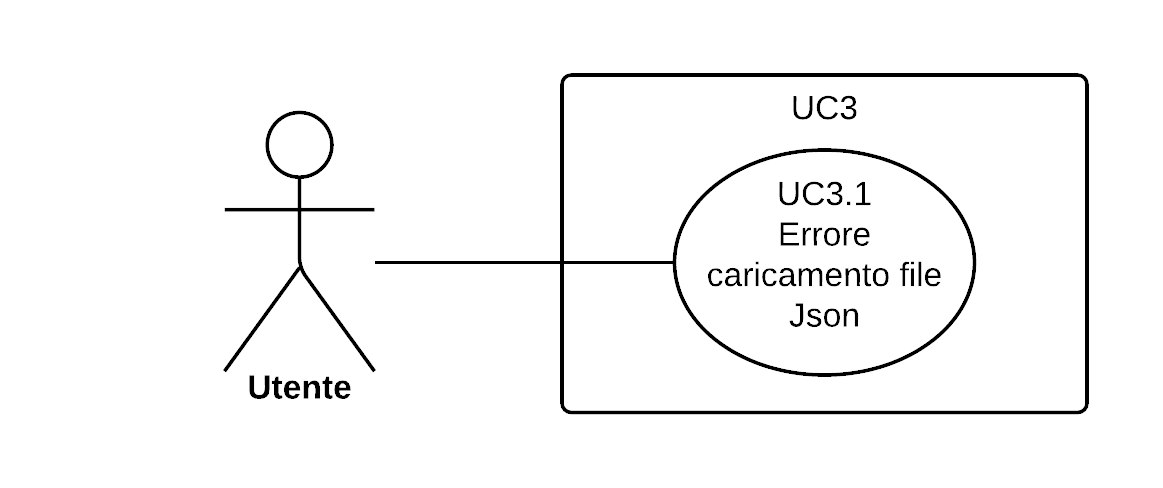
\includegraphics[width=\textwidth]{../img/UC3.png}
		\caption{UC3: File Browser}
	\end{figure}
	\UserCase
	{UC3}
	{Utente}
	{Non previsto}
	{L'attore deve navigare nel file system alla ricerca di un file o di una cartella}
	{L'attore deve selezionare un file o raggiungere una cartella}
	{Viene selezionato il file da caricare o la cartella in cui salvare}
	{
		\begin{itemize}
			\item{} L'attore naviga nel \glossario{file system}{file system} cercando un file o una cartella \refer{UC3.1}
			\item{} L'attore seleziona un file \refer{UC3.2}
		\end{itemize}
	}
	{Non previsti}
	
	\section{UC3.1: Navigazione nel file system}
	\begin{figure}[H]
		\centering
		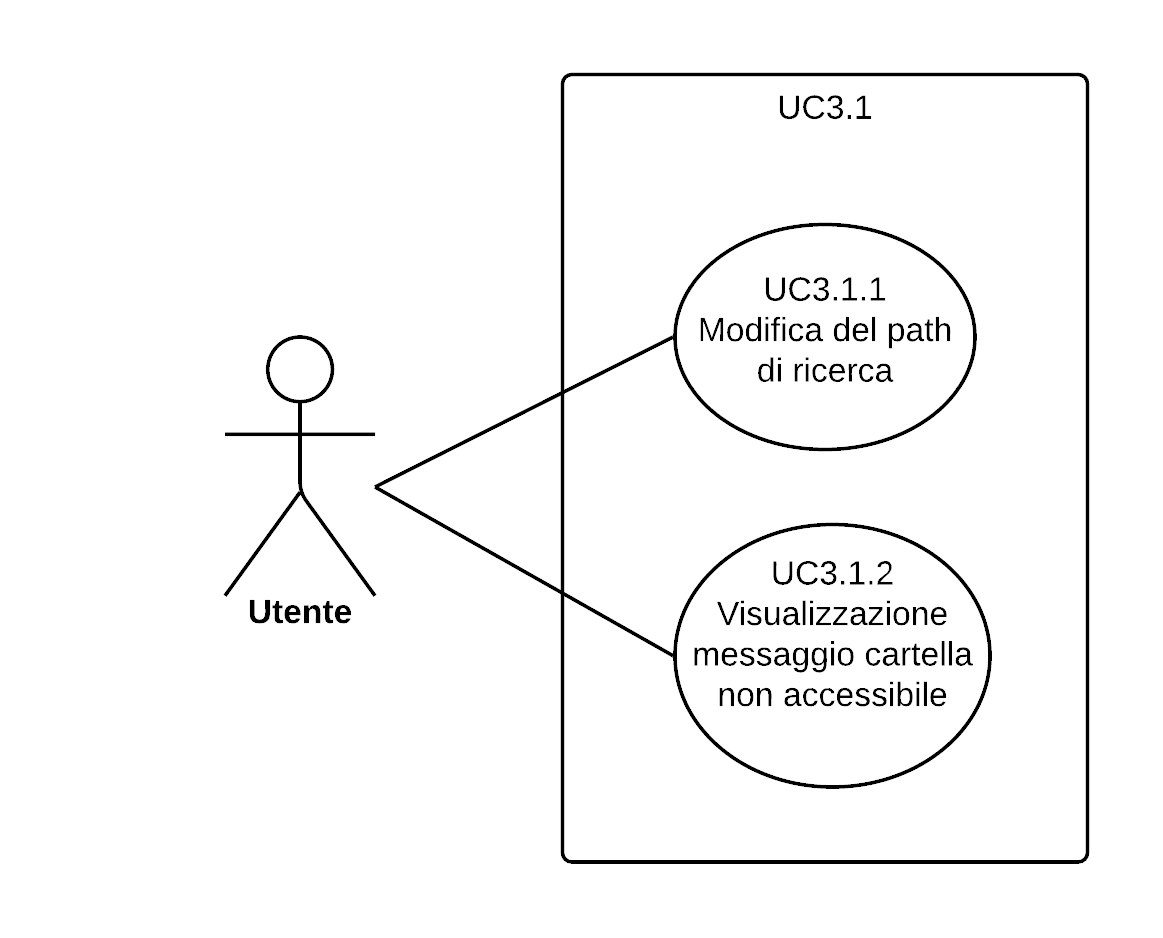
\includegraphics[width=\textwidth]{../img/UC3_1.png}
		\caption{UC3.1: Navigazione nel file system}
	\end{figure}
	\UserCase
	{UC3.1}
	{Utente}
	{Non previsto}
	{L'attore può navigare nel file system per cercare un file o una cartella}
	{L'applicazione ha accesso al file system}
	{La directory selezionata è quella desiderata dall'utente}
	{
		L'attore cerca un file o una cartella spostandosi tra le
		certelle del file system
	}
	{Il file o la cartella cercati non esistono. La ricerca viene annullata}	
	
	\section{UC3.1.1: Modifica del path di ricerca}
	\UserCase
	{UC3.1.1}
	{Utente}
	{Non previsto}
	{L'attore può modificare il path nel quale cercare selezionando una cartella o tornando al passo precedente}
	{L'attore sta navigando nel file system \refer{UC3.1}}
	{Il path nel quale cercare il documento è stato modificato}
	{L'attore si sposta nel file system accedendo ad una cartella o tornando alla directory padre}
	{Se non è possibile accedere alla cartella viene visualizzato un messaggio di errore \refer{UC3.1.2}}
	
	\section{UC3.1.2: Visualizzazione messaggio cartella non accessibile}
	\UserCase
	{UC3.1.2}
	{Utente}
	{Non previsto}
	{L'applicazione visualizza un messaggio di errore per avvisare l'attore che la cartella selezionata non è accessibile}
	{L'attore sta navigando nel file system \refer{UC3.1}}
	{Il path di ricerca corrisponde ad una cartella accessibile}
	{L'attore cerca di accedere ad una cartella che non può essere visitata e l'applicazione visualizza un messaggio di errore}
	{Non previsti}

	\section{UC3.2: Scelta di un file}
	\begin{figure}[H]
		\centering
		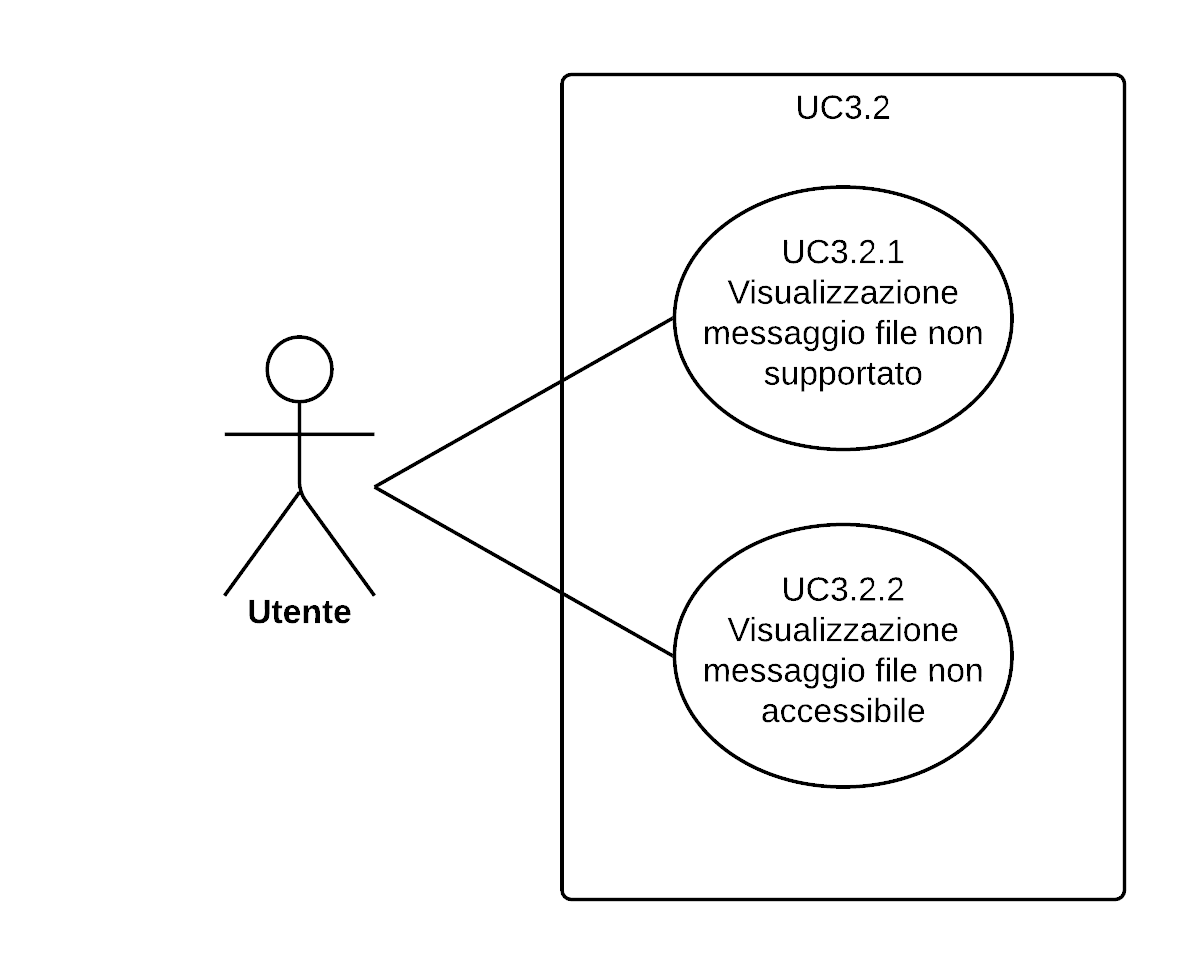
\includegraphics[width=\textwidth]{../img/UC3_2.png}
		\caption{UC3.2: Scelta di un file}
	\end{figure}
\UserCase
{UC3.2}
{Utente}
{Non previsto}
{L'attore sceglie un file tra quelli disponibili nella directory di ricerca}
{L'attore si trova in una directory nella quale c'è almeno un file da selezionare}
{Un file è stato selezionato}
{
	\begin{itemize}
		\item{} L'attore clicca sul file
		\item{} Il file selezionato viene evidenziato
	\end{itemize}
}
{Viene visualizzato un messaggio di errore se il file selezionato non ha un formato supportato \refer{UC3.2.1} o se l'applicazione non ha i permessi per accedere al file \refer{UC3.2.2}}

\section{UC3.2.1:
Visualizzazione messaggio file non supportato}
\UserCase
{UC3.2.1}
{Utente}
{Non previsto}
{L'applicazione visualizza un messaggio di errore per avvisare l'attore che il file non è supportato}
{L'attore ha selezionato un file \refer{UC3.2}}
{Il file non viene importato e l'attore può continuare la navigazione nel file system}
{L'attore ha selezionato un file con formato non supportato e viene visualizzato un messaggio di errore}
{Non previsti}

\section{UC3.2.2:
Visualizzazione messaggio file non accessibile}
\UserCase
{UC3.2.2}
{Utente}
{Non previsto}
{L'applicazione visualizza un messaggio di errore per avvisare l'attore che il file non è accessibile}
{L'attore ha selezionato un file \refer{UC3.2}}
{Il file non viene importato e l'attore può continuare la navigazione nel file system}
{L'attore ha selezionato un file al quale l'applicazione non può accedere e viene visualizzato un messaggio di errore}
{Non previsti}



\section{UC4: Salvataggio Audio Prodotto}
\begin{figure}[H]
	\centering
	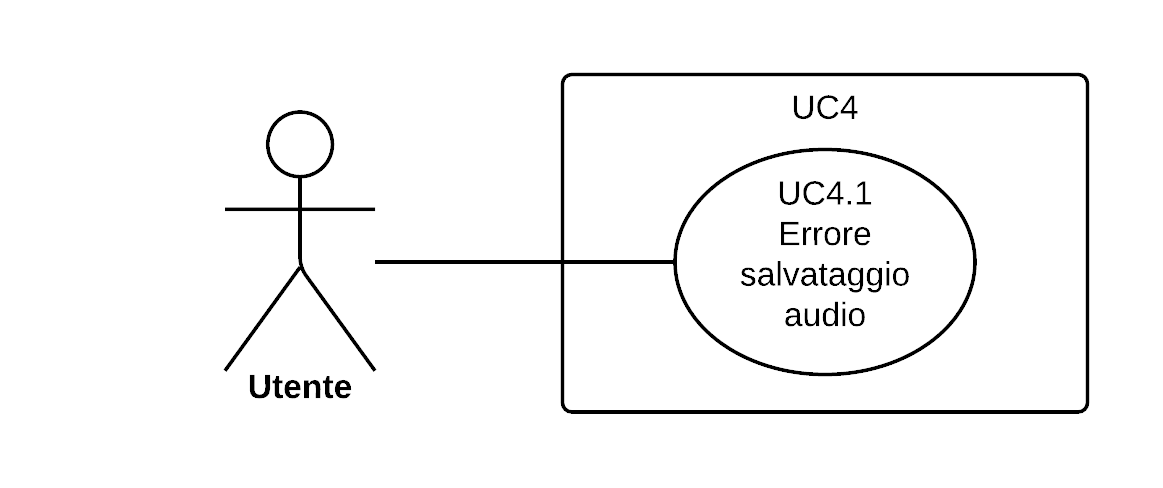
\includegraphics[width=\textwidth]{../img/UC4.png}
	\caption{UC4: Salvataggio Audio Prodotto}
\end{figure}
\UserCase
{UC4}
{Utente}
{Non previsto}
{L'attore vuole salvare l'audio prodotto}
{Speect è inizializzato \refer{UC2}}
{L'audio è salvato in un file}
{
		\begin{itemize}
		\item{} Viene aperto il file browser \refer{UC3}
		\item{} L'attore si sposta nella cartella di destinazione \refer{UC3.1}
		\item{} L'attore scrive il nome del file nella barra di testo
		\item{} L'attore preme su Salva 
		\item{} Speect compila producendo il file desiderato
		\item{} Il file viene salvato nella destinazione con estensione .WAV
		\end{itemize}
}
{Avviene un errore durante il salvataggio dell'audio e l'attore visualizza il messaggio di errore relativo \refer{UC4.1}}
		
\section{UC4.1: Errore Salvataggio Audio}
\UserCase
{UC4.1}
{Utente}
{Non previsto}
{Avviene un errore durante il salvataggio dell'audio}
{L'attore ha cercato di salvare il file audio prodotto} 
{Viene visualizzato l'errore e nessuna operazione viene eseguita}
{L'attore ha cercato di salvare il file audio prodotto e viene visualizzato un messaggio di errore}
{Non previsti}

\section{UC5: Uscita Applicazione}
\begin{figure}[H]
	\centering
	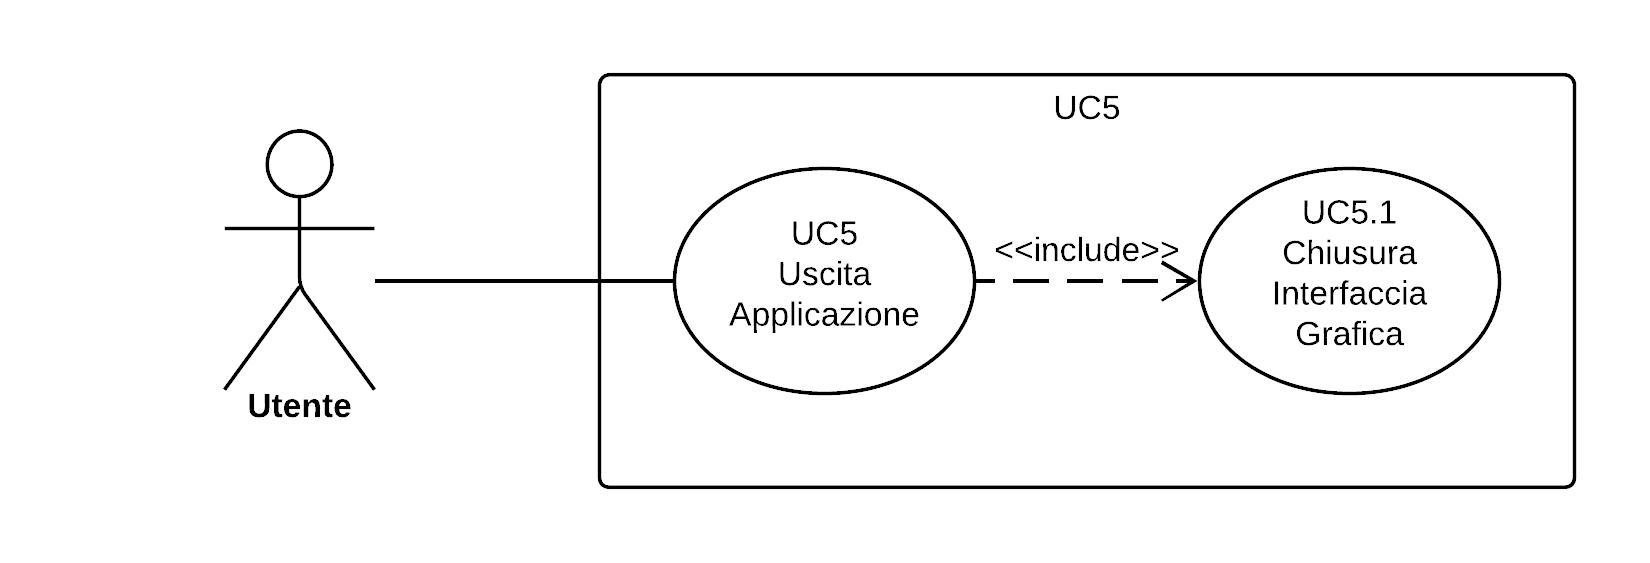
\includegraphics[width=\textwidth]{../img/UC5.png}
	\caption{UC5: Uscita Applicazione}
\end{figure}
\UserCase
{UC5}
{Utente}
{Non previsto}
{L'attore vuole chiudere l'applicazione}
{Viene confermata la chiusura dell'applicazione \refer{UC5.1}}
{L'applicazione viene terminata}
{Chiusura dell'applicazione}
{L'attore annulla la chiusura dell'applicazione \refer{UC5.1}}

\section{UC5.1: Chiusura Interfaccia Grafica}
\UserCase
{UC5.1}
{Utente}
{Non previsto}
{L'attore visualizza una finestra di conferma}
{L'applicazione è in esecuzione}
{L'attore conferma la chiusura dell'applicazione}
{L'attore visualizza una finestra di conferma e richiede la chiusura dell'applicazione}
{L'attore visualizza una finestra di conferma e annulla la chiusura dell'applicazione}

\section{UC6: Modifica Utterance Type}
\begin{figure}[H]
	\centering
	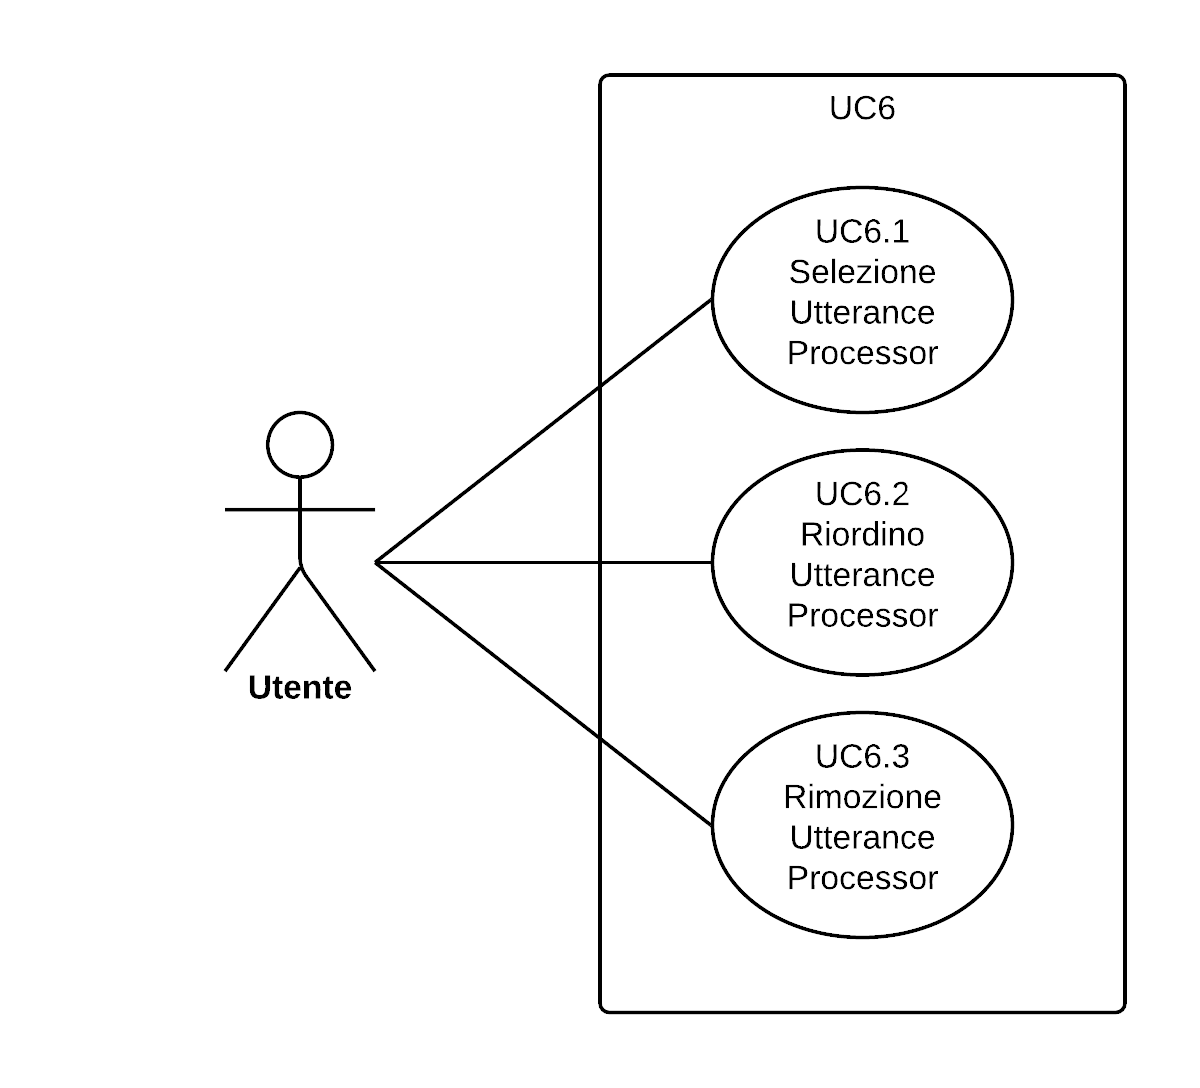
\includegraphics[width=\textwidth]{../img/UC6.png}
	\caption{UC6: Modifica Utterance Type}
\end{figure}
\UserCase
{UC6}
{Utente}
{Non previsto}
{L'attore vuole modificare l'Utterance Type}
{E' presente almeno un'Utterance Type e questo è selezionato \refer{UC12}}
{L'Utterance Type è stato modificato e il file JSon viene aggiornato}
{
	\begin{itemize}
		\item{} L'attore seleziona un Utterance Processor
		\item{} L'attore riordina o rimuove l'Utterance Processor	
		\item{} Le operazioni vengono eseguite	
		\item{} Il file JSon relativo viene aggiornato		
	\end{itemize}
}
{Non previsti}

\section{UC6.1: Selezione Utterance Processor}
\UserCase
{UC6.1}
{Utente}
{Non previsto}
{L'attore vuole selezionare un Utterance Processor per spostarlo}
{Un file JSon è stato caricato correttamente \refer{UC2}}
{Vengono visualizzati i bottoni per modificare tale Utterance Processor}
{
	\begin{itemize}
		\item{} L'attore clicca sul nome dell'Utterance Processor
		\item{} Vengono visualizzati due bottoni che permettono lo spostamento grafico del Utterance Processor \refer{UC6.2} e un bottone che ne permette la rimozione \refer{UC6.3} 		
	\end{itemize}
}
{Non previsti}

\section{UC6.2: Riordino Utterance Processor}
\UserCase
{UC6.2}
{Utente}
{Non previsto}
{L'attore vuole cambiare l'ordine degli Utterance Processor}
{L'attore ha selezionato un Utterance Processor \refer{UC6.1}}
{Il file JSon viene aggiornato}
{
	\begin{itemize}
		\item{} L'attore clicca sull'Utterance Processor \refer{UC6.1}
		\item{} L'attore riordina tramite i pulsanti forniti	
		\item{} Le operazioni vengono eseguite
		\item{} Se esisteva un grafo, esso non viene modificato
		
	\end{itemize}
}
{Non previsti}

\section{UC6.3: Rimozione Utterance Processor}
\UserCase
{UC6.3}
{Utente}
{Non previsto}
{L'attore vuole rimuovere un Utterance Processor}
{L'attore ha selezionato un Utterance Processor \refer{UC6.1}}
{Il file JSon viene aggiornato}
{
	\begin{itemize}
		\item{} L'attore clicca sull'Utterance Processor \refer{UC6.1}
		\item{} L'attore lo rimuove tramite il pulsante fornito	
		\item{} L'operazione viene eseguita
		\item{} Se esisteva un grafo, esso non viene modificato
		
	\end{itemize}
}
{Non previsti}

\section{UC7: Esecuzione Speect}
\begin{figure}[H]
	\centering
	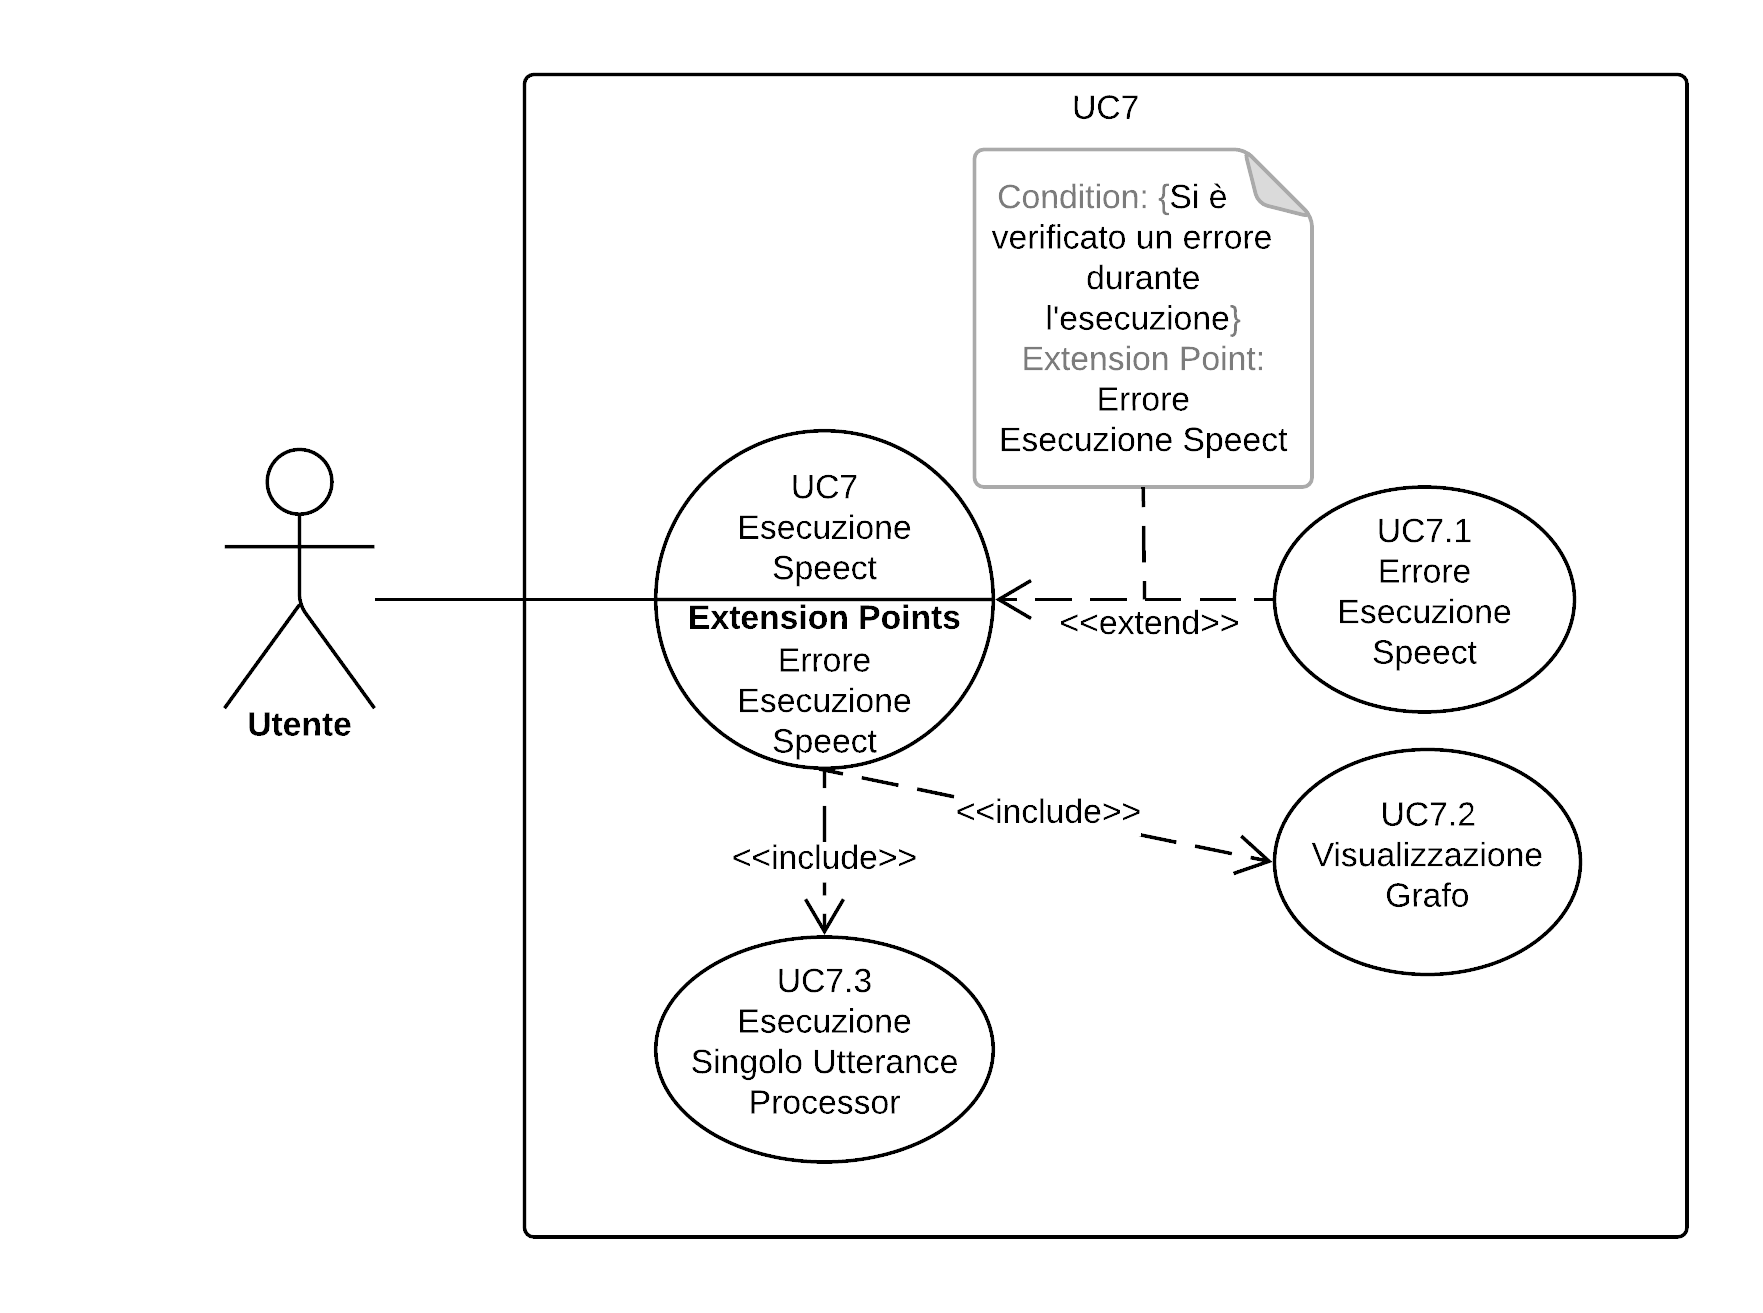
\includegraphics[width=\textwidth]{../img/UC7.png}
	\caption{UC7: Esecuzione}
\end{figure}
\UserCase
{UC7}
{Utente}
{Non previsto}
{L'attore vuole eseguire Speect}
{Il file JSon è stato caricato correttamente \refer{UC2}}
{Speect elabora il testo selezionato e viene visualizzato il grafo}
{\begin{itemize}
		\item{} L'attore seleziona l'Utterance Type \refer{UC12}
		\item{} L'attore compila il campo di testo o inserisce un grafo hrg
		\item{} L'attore preme sul tasto di esecuzione
		\item{} Vengono eseguiti gli Utterance Processor designati dall'Utterance Type \refer{UC7.3}
		\item{} Viene mostrato il grafo risultante dall'esecuzione \refer{UC7.2}
	\end{itemize}
}
{Speect ha fallito l'esecuzione e l'attore visualizza un messaggio di errore \refer{UC7.1}}

\section{UC7.1: Errore Esecuzione Speect}
\UserCase
{UC7.1}
{Utente}
{Non previsto}
{L'attore visualizza a schermo l'errore di esecuzione di Speect}
{Speect ha fallito l'esecuzione}
{Viene visualizzato un messaggio di errore}
{L'attore ha provato ad eseguire Speect e viene visualizzato un messaggio di errore}
{Non previsti}

\section{UC7.2: Visualizzazione Grafo}
\UserCase
{UC7.2}
{Utente}
{Non previsto}
{L'attore visualizza il grafo}
{Speect ha terminato l'esecuzione con successo \refer{UC7}}
{Viene visualizzato a schermo un grafo corretto con almeno un nodo cliccabile}
{
	L'attore visualizza il grafo corretto e può modificarlo \refer{UC13}
}
{Non previsti}

\section{UC7.3: Esecuzione Singolo Utterance Processor}
\UserCase
{UC7.3}
{Utente}
{Non previsto}
{Speect esegue un singolo Utterance Processor}
{Un Utterance Type è stato selezionato \refer{UC12} }
{Viene eseguito l'Utterance Processor partendo dal grafo già presente o dal campo di testo scritto}
{
	\begin{itemize}
		\item{} L'attore seleziona l'Utterance Processor \refer{UC6.1}
		\item{} L'attore può compilare il campo di testo
		\item{} L'attore preme sul tasto di esecuzione per il singolo processor \ref{fig:GUI}
	\end{itemize}
}
{Speect ha fallito l'esecuzione}

\section{UC8: Esportazione Grafo}
\begin{figure}[H]
	\centering
	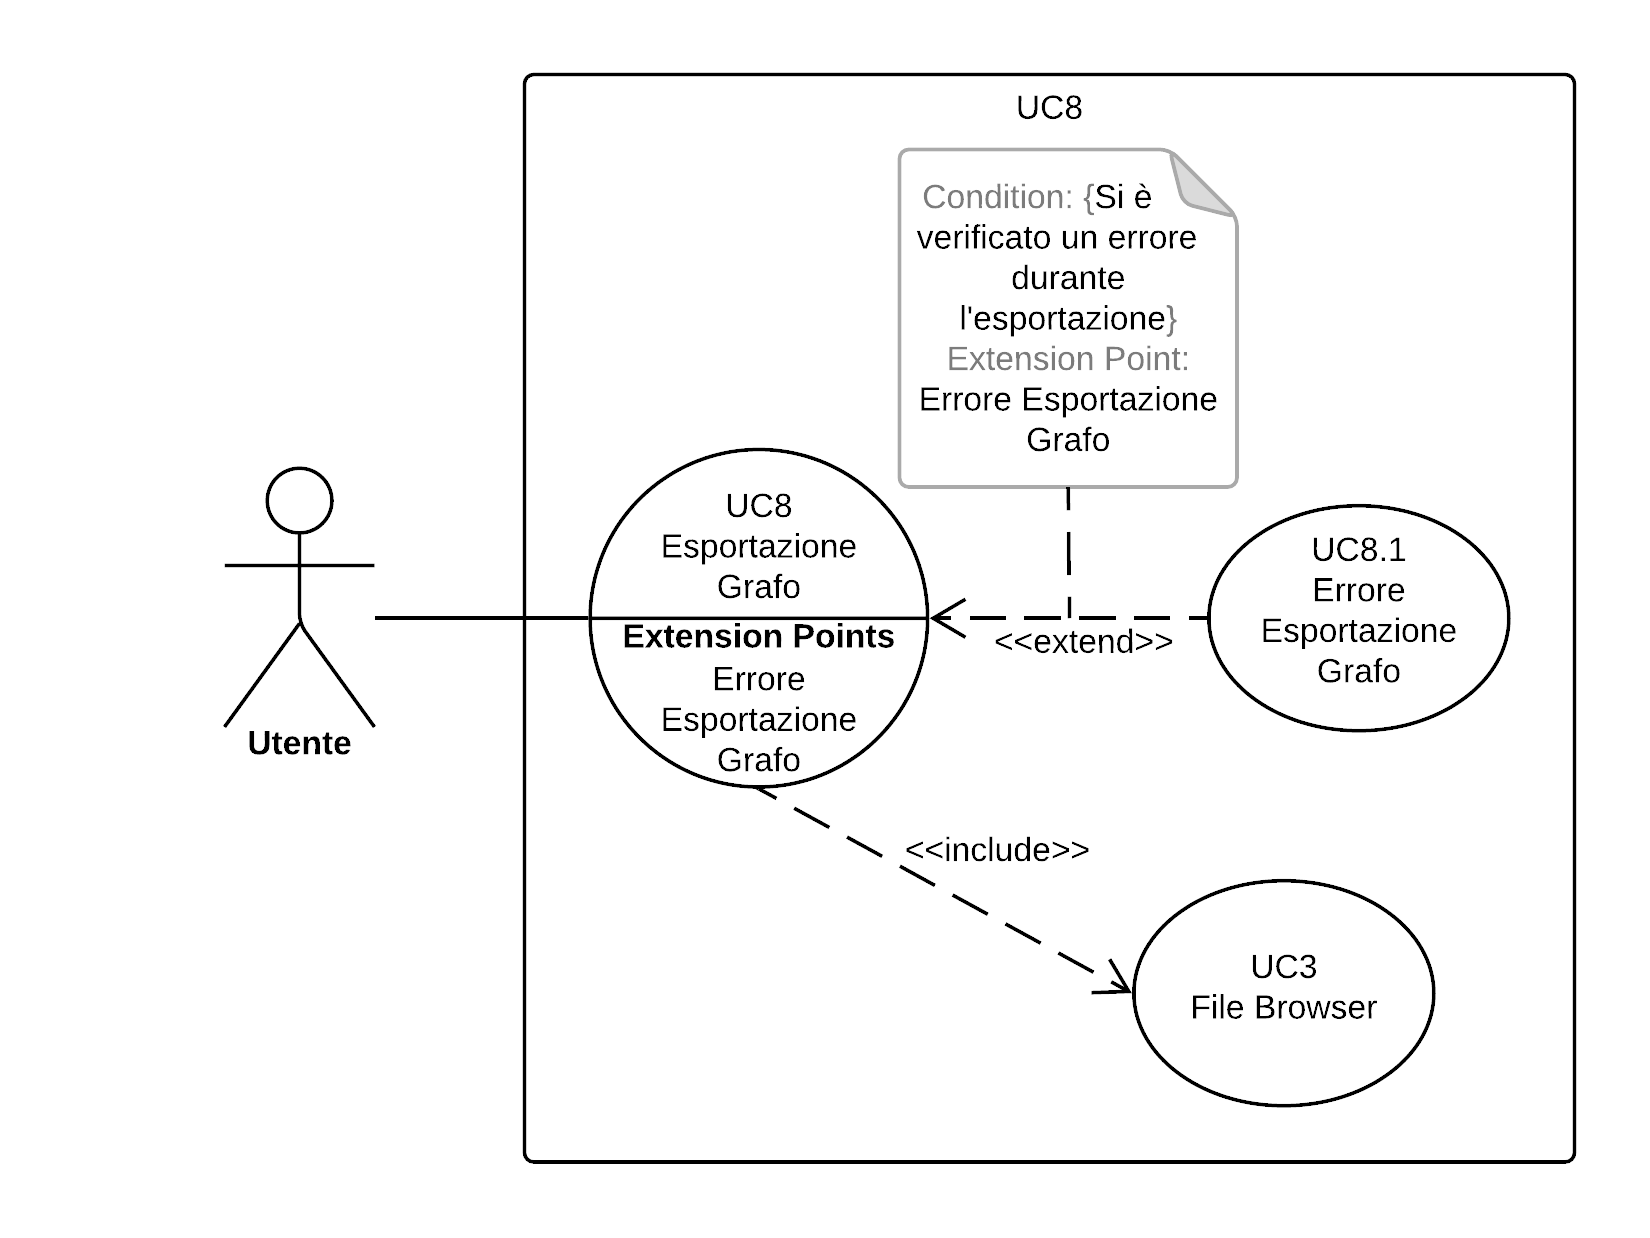
\includegraphics[width=\textwidth]{../img/UC8.png}
	\caption{UC8: Esportazione Stato del Grafo}
\end{figure}
\UserCase
{UC8}
{Utente}
{Non previsto}
{L'attore vuole esportare il grafo visualizzato}
{Esiste un grafo esportabile}
{Il grafo viene esportato in file}
{
	\begin{itemize}
			\item{} Viene aperto il file browser \refer{UC3}
			\item{} L'attore si sposta nella cartella in cui salvare il grafo \refer{UC3.1}
			\item{} L'attore scrive il nome del file nella barra di testo
			\item{} L'attore preme su Salva Grafo
	\end{itemize}
}
{L'esportazione fallisce e l'attore visualizza un messaggio di errore \refer{UC8.1}}

\section{UC8.1: Errore Esportazione Grafo}
\UserCase
{UC8.1}
{Utente}
{Non previsto}
{Avviene un errore durante l'esportazione}
{L'esportazione del grafo è fallita}
{Viene visualizzato un messaggio di errore e nessuna operazione viene eseguita}
{L'esportazione del grafo è fallita e viene visualizzato un messaggio di errore}
{Non previsti}

\section{UC9: Importazione Grafo}
\begin{figure}[H]
	\centering
	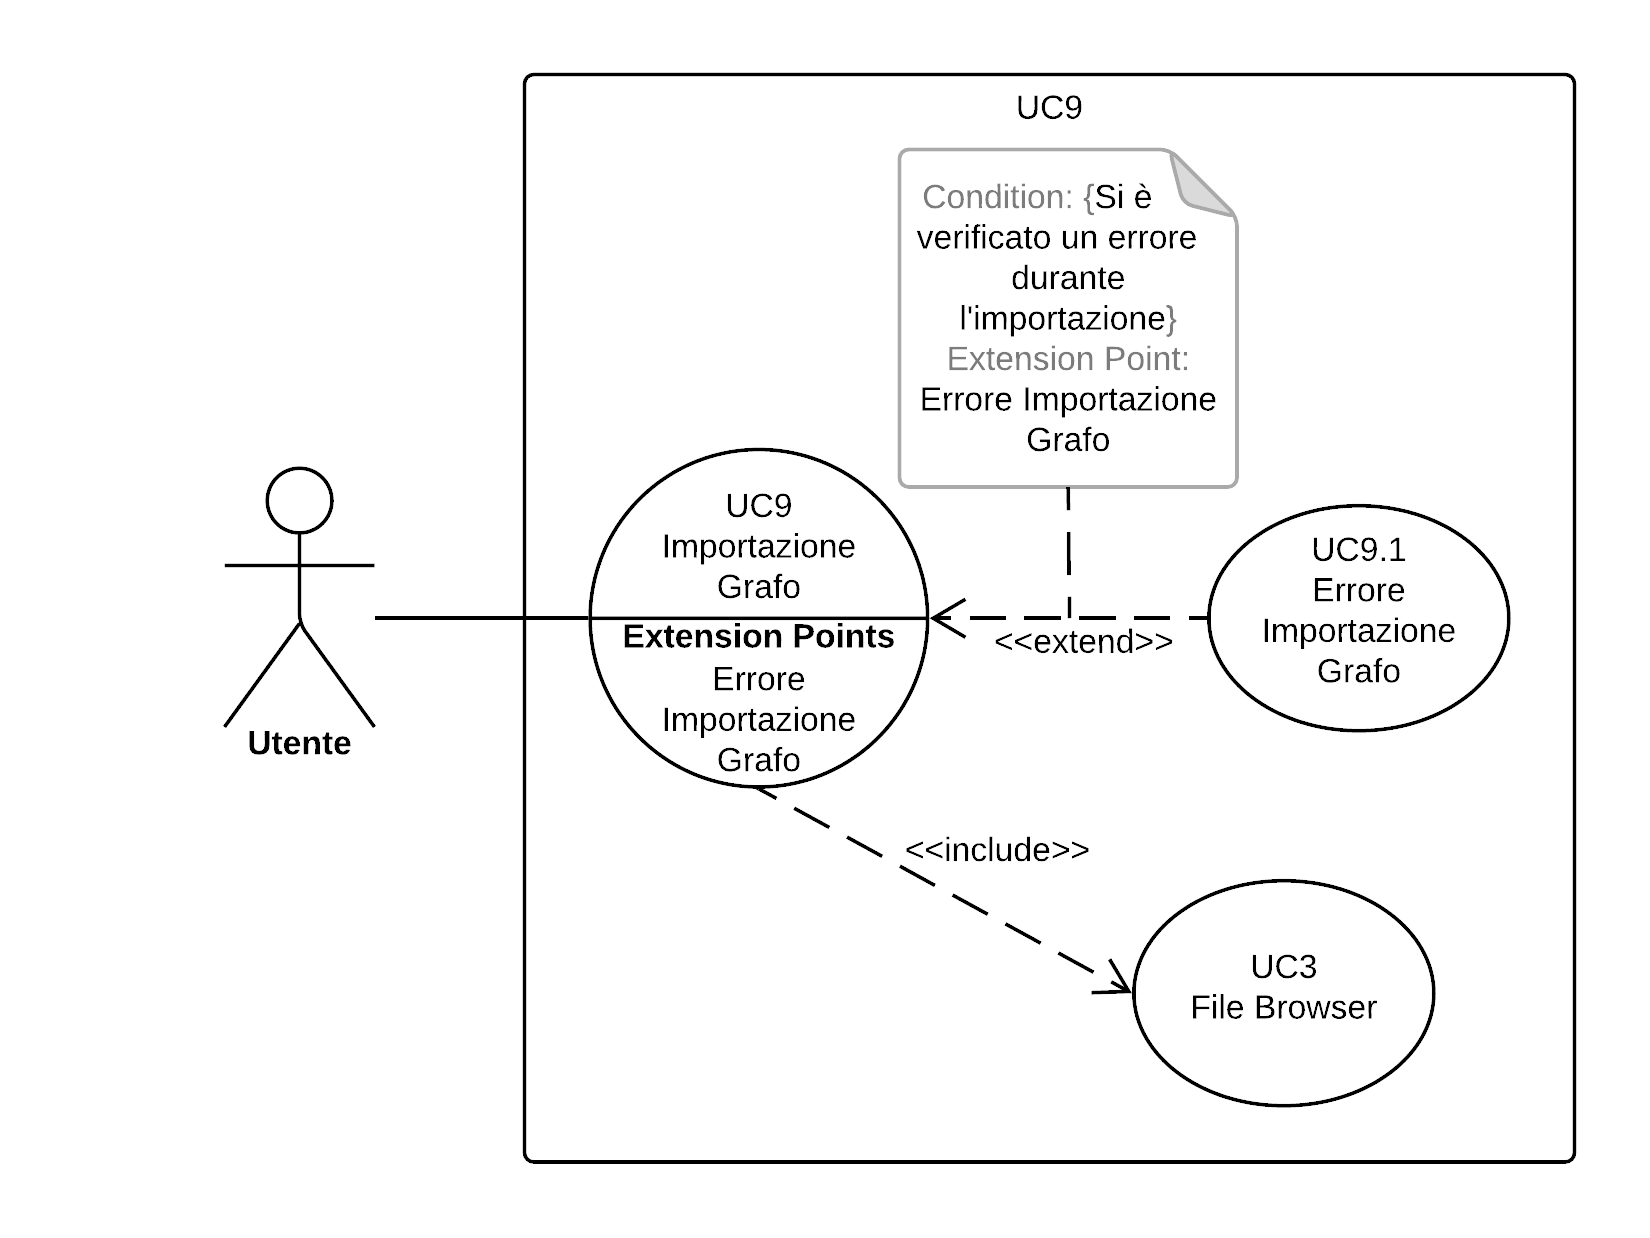
\includegraphics[width=\textwidth]{../img/UC9.png}
	\caption{UC9: Importazione Grafo}
\end{figure}
\UserCase
{UC9}
{Utente}
{Non previsto}
{L'attore vuole importare un grafo}
{Esiste un grafo e l'attore ha cliccato Carica Grafo}
{Il grafo viene importato da file}
{
	\begin{itemize}
			\item{} Viene aperto il file browser \refer{UC3}
			\item{} L'attore seleziona il file da importare \refer{UC3.2}
			\item{} L'attore preme su Apri Grafo
	\end{itemize}
}
{L'importazione fallisce e l'attore visualizza un messaggio di errore \refer{UC9.1}}

\section{UC9.1: Errore Importazione Grafo}
\UserCase
{UC9.1}
{Utente}
{Non previsto}
{Avviene un errore durante l'importazione}
{L'importazione del grafo è fallita}
{Viene visualizzato l'errore e nessuna operazione viene eseguita}
{L'importazione del grafo è fallita e viene visualizzato un messaggio di errore}
{Non previsti}

\section{UC10: Ricerca Path}
\begin{figure}[H]
	\centering
	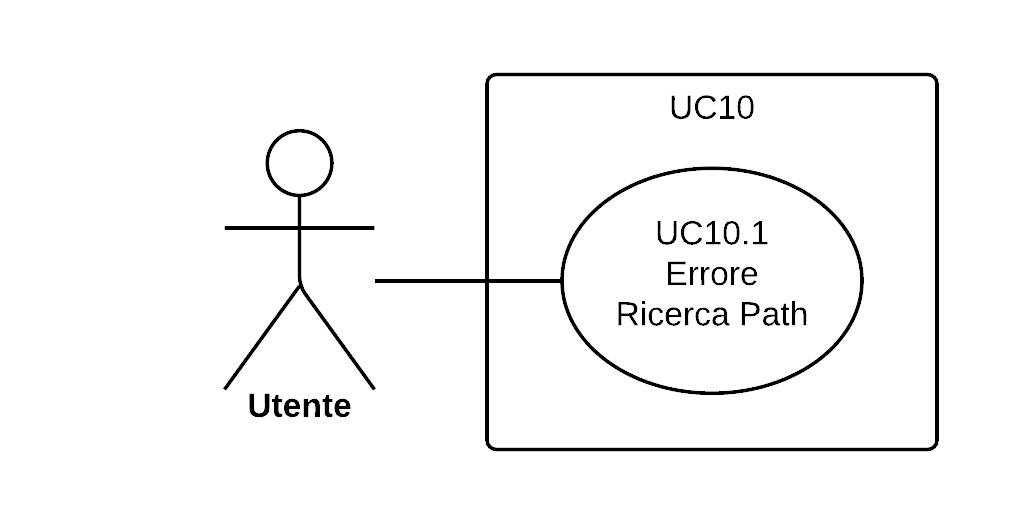
\includegraphics[width=\textwidth]{../img/UC10.png}
	\caption{UC10: Ricerca Path}
\end{figure}
\UserCase
{UC10}
{Utente}
{Non previsto}
{L'attore vuole cercare un nodo tramite un percorso nel grafo}
{Esiste un grafo corretto, l'attore ha selezionato un nodo e premuto Ricerca Path nel menu File}
{Se il path porta ad un nodo definito, esso viene evidenziato \refer{UC7.2.1}}
{
	\begin{itemize}
		\item{} Viene visualizzata una finestra con una casella di testo e un pulsante
		\item{} L'attore inserisce il percorso da cercare
		\item{} L'attore preme il pulsante di Ricerca
		\item{} Se il percorso inizia dal nodo selezionato e finisce in un nodo esistente, il nodo di arrivo viene evidenziato \refer{UC7.2.1}
 	\end{itemize}
}
{Il percorso inserito dall'attore non è corretto e viene visualizzato un errore \refer{UC10.1}}

\section{UC10.1: Errore Ricerca Path}
\UserCase
{UC10.1}
{Utente}
{Non previsto}
{L'attore vuole cercare un nodo tramite un percorso nel grafo}
{Il percorso inserito dall'attore è sintatticamente errato}
{Viene visualizzato l'errore a schermo e si riapre la finestra di Ricerca \refer{UC10}}
{Il percorso inserito dall'attore non è corretto e viene visualizzato un messaggio di errore}
{Non previsti}

\section{UC11: Salvataggio modifiche file JSon}
\begin{figure}[H]
	\centering
	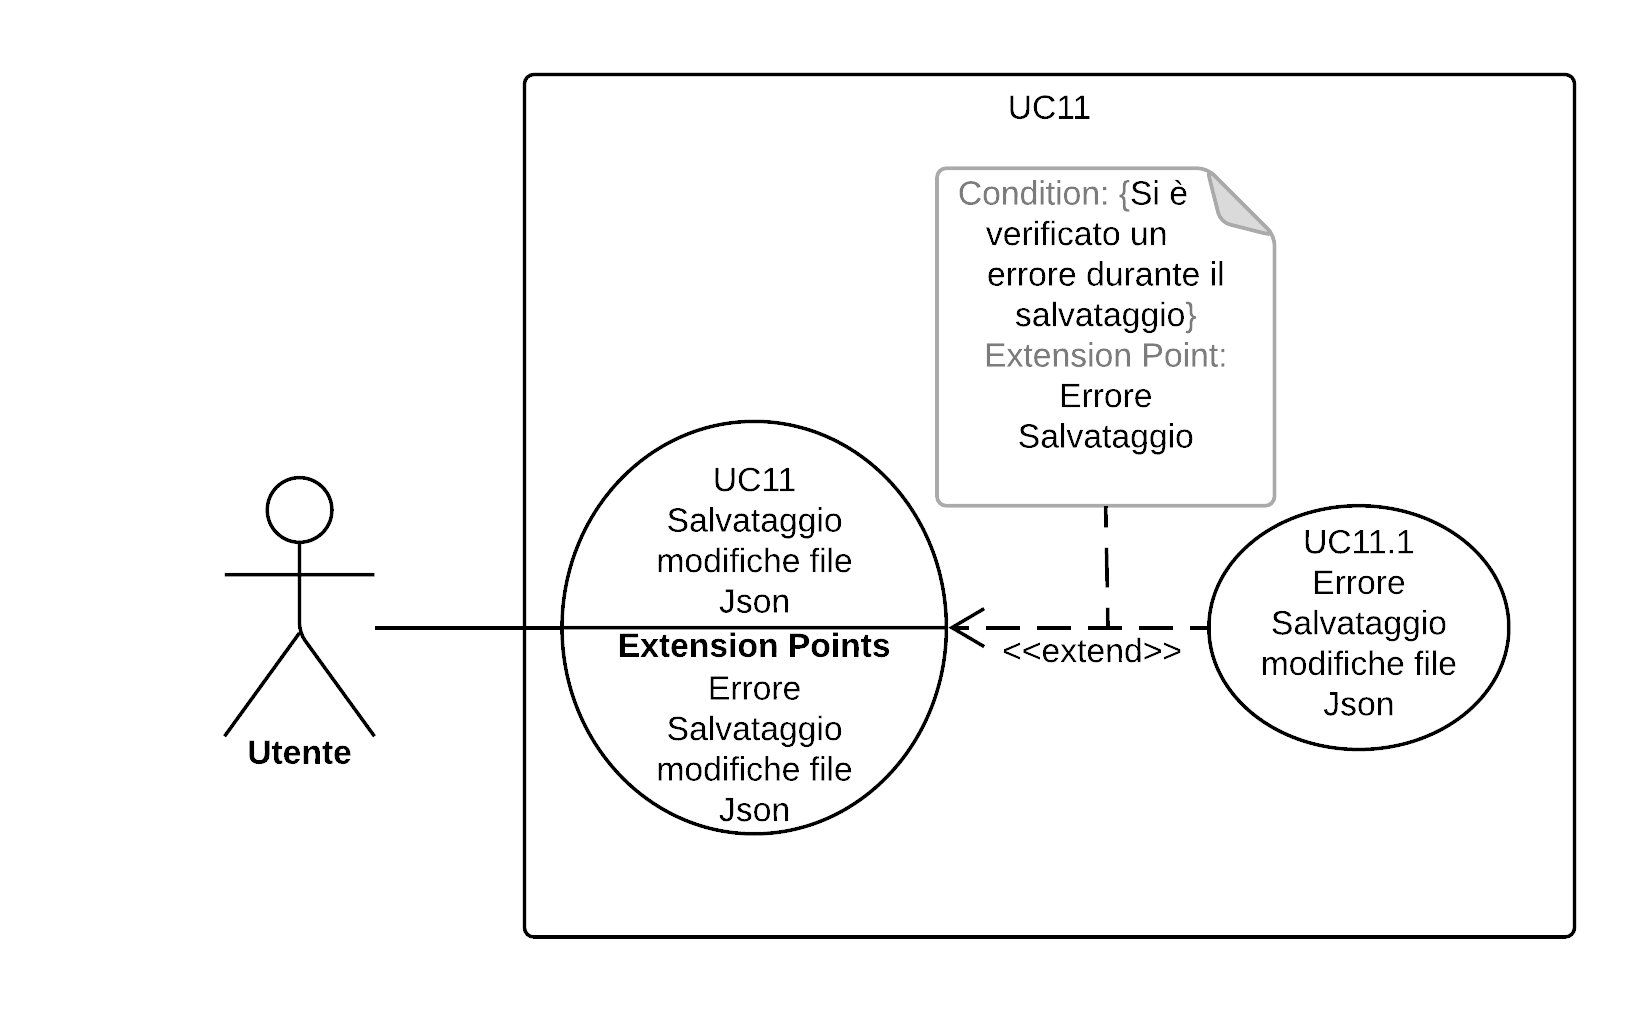
\includegraphics[width=\textwidth]{../img/UC11.png}
	\caption{UC11: Salvataggio modifiche file JSon}
\end{figure}
\UserCase
{UC11}
{Utente}
{Non previsto}
{L'attore ha modificato gli Utterance Processor e vuole salvare il nuovo file JSon}
{Esiste un file Json correttamente caricato \refer{UC2} e l'attore ha modificato gli Utterance Processor \refer{UC6.2} \refer{UC6.3}}
{Le modifiche vengono salvate}
{
	\begin{itemize}
		\item{} L'attore apre il menu File \refer{UC1}
		\item{} L'attore preme su Salva File JSon
	\end{itemize}
}
{L'operazione di salvataggio fallisce e viene visualizzato un errore \refer{UC11.1}}

\section{UC11.1: Errore Salvataggio modifiche file JSon}
\UserCase
{UC11.1}
{Utente}
{Non previsto}
{L'attore ha provato a salvare il file JSon}
{L'operazione di salvataggio fallisce}
{Viene visualizzato l'errore e nessuna operazione viene eseguita}
{L'operazione di salvataggio fallisce e viene visualizzato un errore}
{Non previsti}

\section{UC12: Selezione Utterance Type}
\UserCase
{UC12}
{Utente}
{Non previsto}
{L'attore vuole selezionare l'Utterance Type desiderato}
{Un file JSon è stato caricato correttamente \refer{UC2}}
{Vengono mostrati gli Utterance Processors utilizzati da Speect per tale Utterance Type}
{
	\begin{itemize}
		\item{} L'attore apre il menu a tendina relativo
		\item{} L'attore clicca sull'Utterance Type desiderato
		\item{} Vengono mostrati a schermo i nomi degli Utterance Processor utilizzati, negli appositi spazi \ref{fig:GUI}		
	\end{itemize}
}
{Non previsti}

\section{UC13: Modifica Grafo}
\begin{figure}[H]
	\centering
	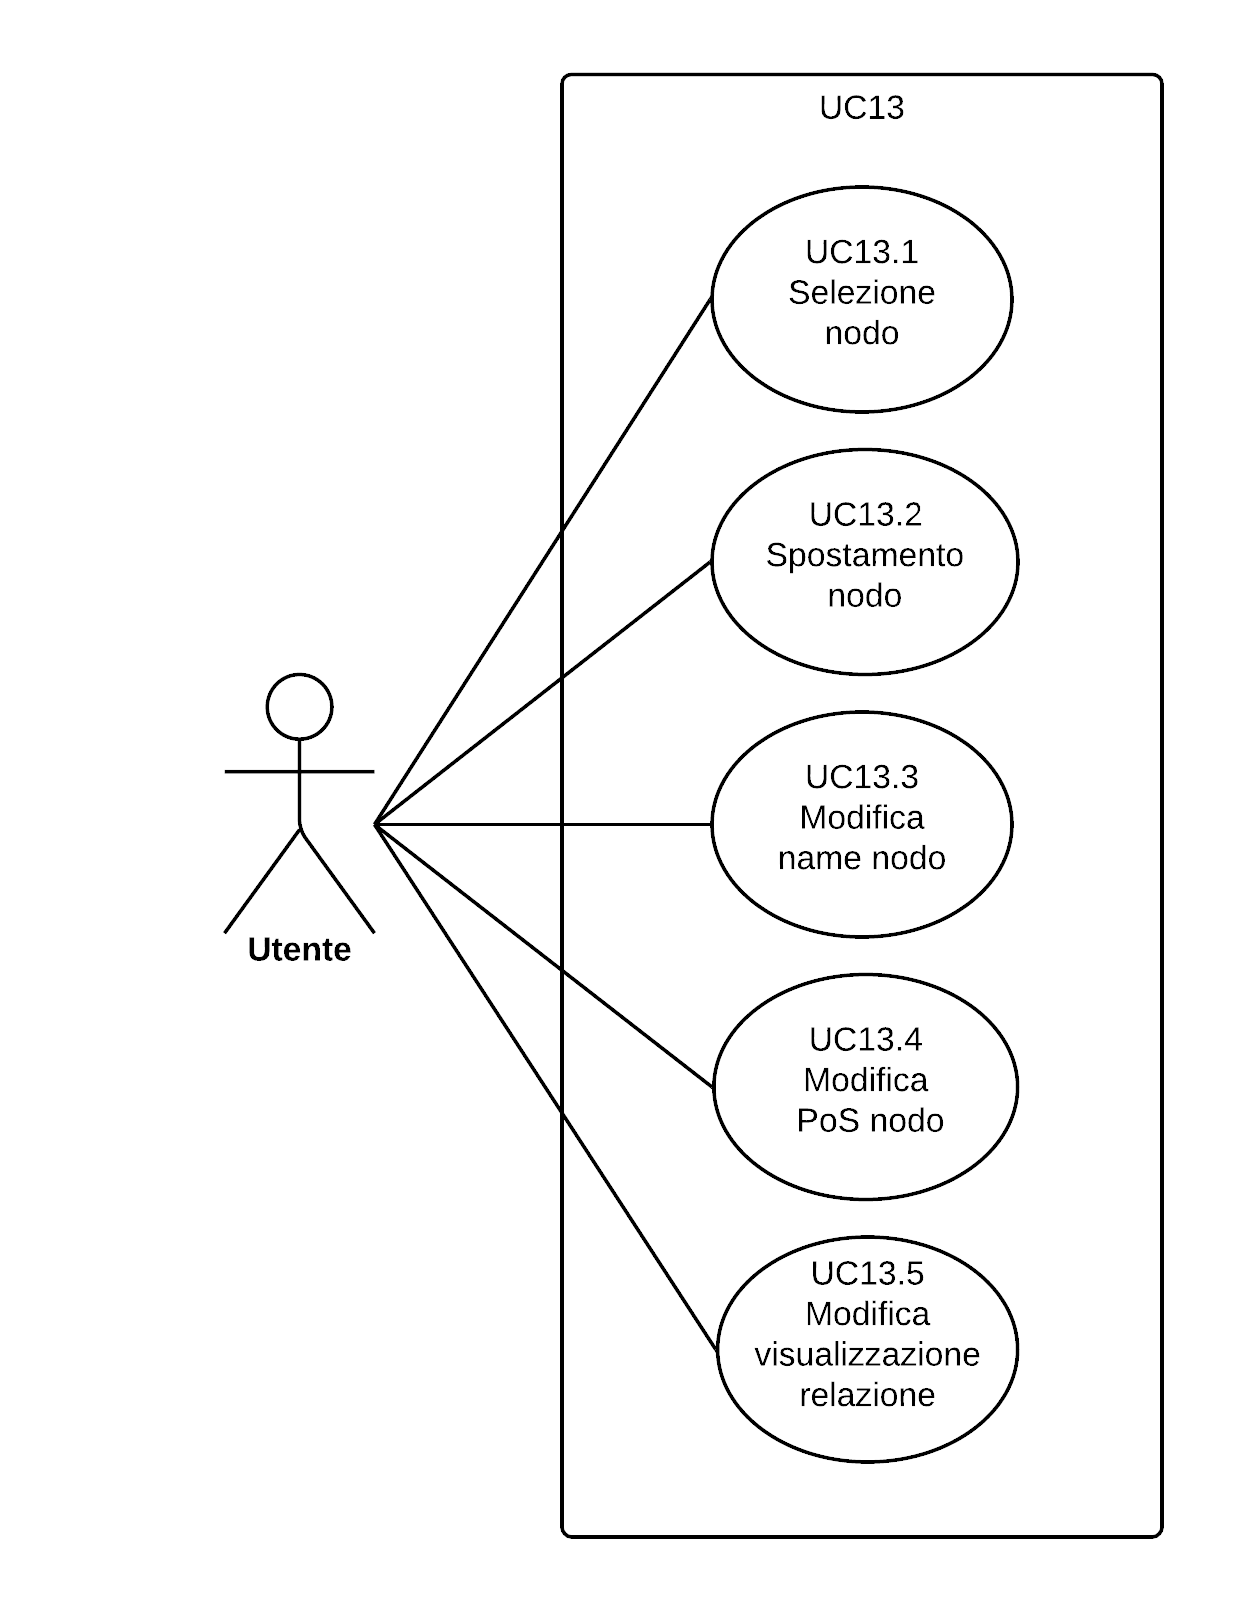
\includegraphics[width=\textwidth]{../img/UC13.png}
	\caption{UC13: Modifica Grafo}
\end{figure}
\UserCase
{UC13}
{Utente}
{Non previsto}
{L'attore vuole modificare il grafo}
{Viene visualizzato a schermo un grafo corretto con almeno un nodo cliccabile \refer{UC7.2}}
{Il grafo è stato modificato}
{
	L'attore per modificare un grafo può:
	\begin{itemize}
		\item{} selezionare un nodo \refer{UC13.1}
		\item{} spostare un nodo \refer{UC13.2}	
		\item{} modificare la visualizzazione delle relazioni \refer{UC13.5}		
	\end{itemize}
}
{Non previsti}

\section{UC13.1: Selezione Nodo}
\UserCase
{UC13.1}
{Utente}
{Non previsto}
{L'attore vuole selezionare un nodo per visualizzarne i dettagli}
{Viene visualizzato a schermo un grafo corretto con almeno un nodo cliccabile \refer{UC7.2}}
{Viene evidenziato il nodo del grafo e vengono mostrate le sue informazioni nella finestra apposita}
{
	\begin{itemize}
		\item{} L'attore clicca una volta sul nodo
		\item{} Il nodo viene evidenziato con un contorno giallo
		\item{} Nel riquadro apposito \ref{fig:GUI} vengono visualizzati i dati del grafo:
		\begin{enumerate}
			\item{} Name
			\item{} Part of Speech
		\end{enumerate}
		\item{} L'attore può modificare il name del nodo selezionato \refer{UC13.3}
		\item{} L'attore può modificare il PoS del nodo selezionato \refer{UC13.4} 
	\end{itemize}
}
{Non previsti}

\section{UC13.2: Spostamento Nodo}
\UserCase
{UC13.2}
{Utente}
{Non previsto}
{L'attore vuole spostare graficamente un nodo}
{Un nodo è selezionato \refer{UC13.1}}
{Il nodo viene spostato}
{
	\begin{itemize}
		\item{} L'attore trascina il nodo cliccando senza rilasciare
		\item{} Il nodo si sposta
		\item{} L'attore rilascia il click
		\item{} Il nodo rimane nella nuova posizione
	\end{itemize}
}
{Non previsti}

\section{UC13.3: Modifica Name Nodo}
\UserCase
{UC13.3}
{Utente}
{Non previsto}
{L'attore vuole modificare il name del nodo selezionato}
{Un nodo è selezionato \refer{UC13.1}}
{Il nodo cambia name}
{
	\begin{itemize}
		\item{} L'attore seleziona la casella di testo del name
		\item{} L'attore cancella il name precedente
		\item{} L'attore rimuove il focus dalla casella di testo
		\item{} Il name viene aggiornato
		\item{} Il grafo viene aggiornato e ristampato a schermo \refer{UC7.2}
	\end{itemize}
}
{Non previsti}

\section{UC13.4: Modifica PoS Nodo}
\UserCase
{UC13.4}
{Utente}
{Non previsto}
{L'attore vuole modificare il PoS del nodo selezionato}
{Un nodo è selezionato \refer{UC13.1}}
{Il nodo cambia PoS}
{
	\begin{itemize}
		\item{} L'attore seleziona la casella di testo del PoS
		\item{} L'attore cancella il PoS precedente
		\item{} L'attore rimuove il focus dalla casella di testo
		\item{} Il PoS viene aggiornato
		\item{} Il grafo viene aggiornato e ristampato a schermo \refer{UC7.2}
	\end{itemize}
}
{Non previsti}

\section{UC13.5: Modifica Visualizzazione Relazione}
\UserCase
{UC13.5}
{Utente}
{Non previsto}
{L'attore vuole filtrare le relazioni del grafo}
{Un Utterance Type è stato scelto \refer{UC12}}
{Vengono mostrati nel grafo tutti i layer di relazione selezionati}
{
	\begin{itemize}
		\item{} L'attore seleziona/deseleziona una select box adiacente ad una relazione
		\item{} La relazione in questione viene visualizzata/nascosta
		\item{} Il grafo viene aggiornato e ristampato a schermo \refer{UC7.2}
	\end{itemize}
}
{Non previsti}

\end{document}
